\begin{figure}[p]
\centering
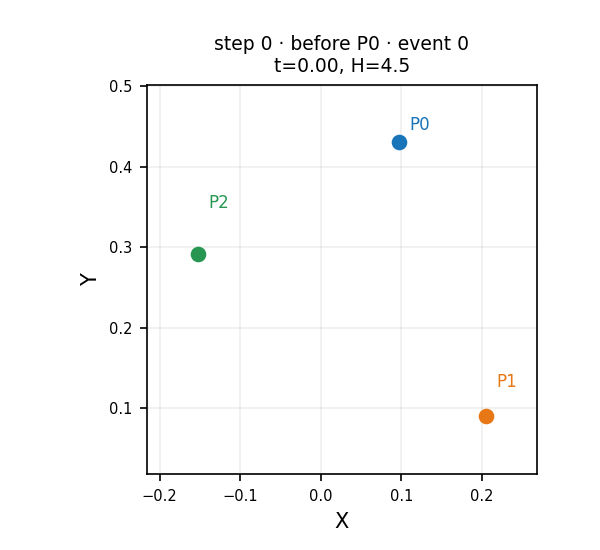
\includegraphics[width=0.485\linewidth,height=0.32\textheight,keepaspectratio]{figures/F03_0.png}
\hfill
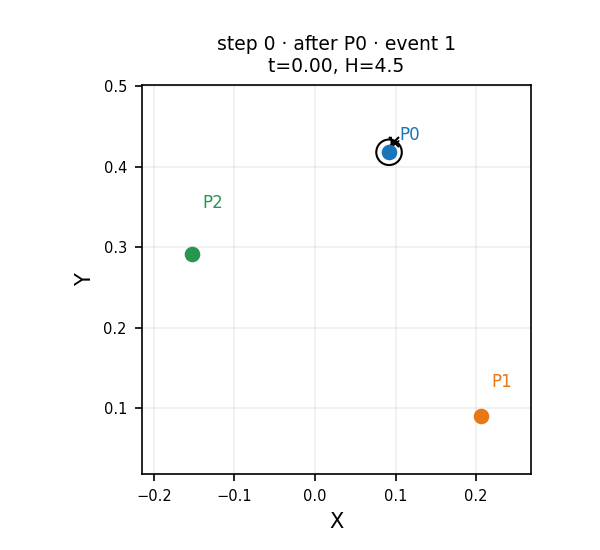
\includegraphics[width=0.485\linewidth,height=0.32\textheight,keepaspectratio]{figures/F03_1.png}
\par\medskip
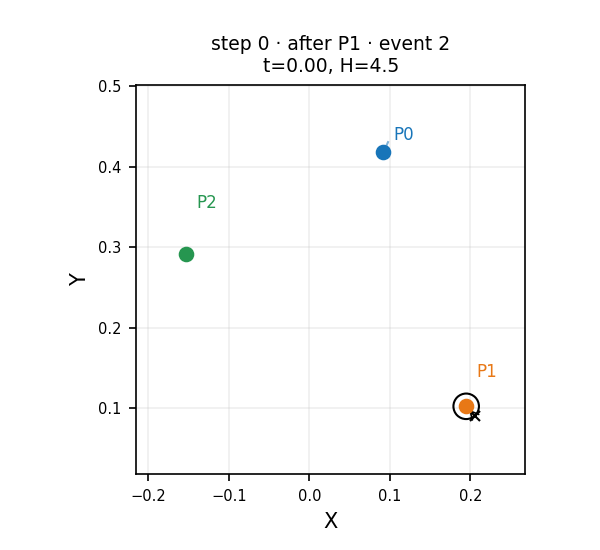
\includegraphics[width=0.485\linewidth,height=0.32\textheight,keepaspectratio]{figures/F03_2.png}
\hfill
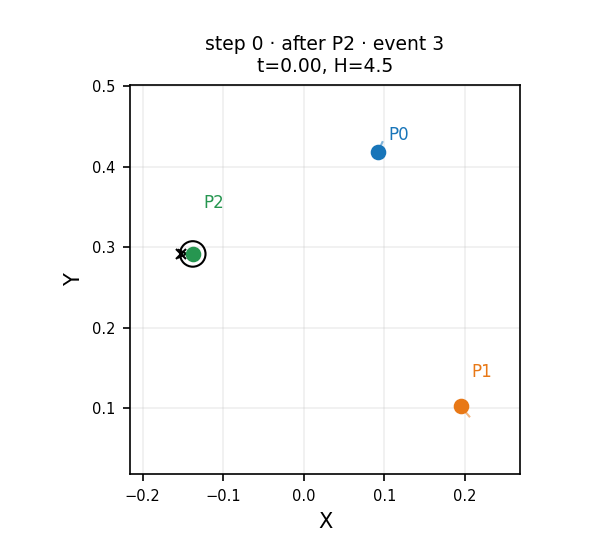
\includegraphics[width=0.485\linewidth,height=0.32\textheight,keepaspectratio]{figures/F03_3.png}
\par\medskip
\caption[The first ordered sweep in the reproduction]{REPRODUCED / OBSERVED, editorial crop. Four panels from the first row of the accepted opening sheet, arranged in reading order: before body 0, after body 0, after body 1, after body 2 (events 0--3). The first panel is the captured initializer; the others are recorded states. X/Y axes retain their original ranges. Arrows connect observed endpoints, not simulated intermediate positions. The source sheet also contains the next two sweeps. \cite{replay01}}
\label{fig:F03}
\end{figure}
